To stress test the FRBR and \textit{Textrad}, neither of which were specially designed for Medieval literature, we explore two cases. The first is a work about the knight Renaut de Montauban. In the 1460s, the work was recomposed in a multi-volume manuscript, which introduces some complexity in relating a text version (\textit{Fassung}) to multiple documents. Second, we underscore the challenge of relating text versions to physical documents through the case of a lost manuscript, which, before being dismembered, allegedly transmitted a version of the \textit{Chanson d'Otinel} and a version of the \textit{Chanson d'Aspremont}. Parts of both are conserved today in two different nineteenth-century collections of Medieval fragments. Through the data model, we want to be able to recognize what scholars argue, which is that the fragments were once transmitted together in a now lost manuscript.

\subsection{\textit{Renaut de Montauban} and multi-volume witnesses}

Let us start with the easier case, concerning a work about the legendary knight Renaut de Montauban. Sahle's \textit{Werke} concept is helpful here in that it defines a work as the ordering of a story's abstract content (\textit{Inhalt}) into a narrative structure. The sequence of events whose order defines the \textit{Work} \textit{Renaut de Montauban} begins with a backstory that contextualizes the main conflict.\footcite[Whether this opening section constitutes a prologue, in alignment with the generic expectations of a prologue for \textit{chansons de geste}, is the subject of scholarly debate.][]{Leverage2000} The narrator explains that four brothers, Aymon, Beuves, Girart, and Doon, once fought together against the emperor Charlemagne. Beuves, who is duke of Aigremont and vassal of Charlemagne, refused some of the duties the emperor had imposed, which provokes the latter's fury. The brothers came to Beuves's aid and joined his conflict with Charlemagne. \textit{Renaut de Montauban} begins with this history because the work's main storyline focuses on how a new generation of brothers, Aymon's sons Renaut, Alard, Guichard, and Richard, again push back against Charlemagne and how the powerful emperor pursues revenge.\footnotemark\footnotetext{Having made peace, duke Aymon brings his four sons, Renaut, Alard, Guichard, et Richard, with him to meet emperor Charlemagne in Paris. After the meeting, Renaut plays chess with Charlemagne's nephew, but the game devolves into a dispute. The knight ultimately slays the nephew. Fearing the emperor's vengeful wrath, Renaut and his brothers flee Paris on the back of a magical horse, Bayard. Adventures ensue.}

In various languages and forms, many people have composed and recomposed the \textit{Work} known by its French title as \textit{Renaut de Montauban}. The earliest instance of such a composition, what Sahle calls the text-as-linguistic-content \brackettext{\textit{sprachlichen Gehalt}} and the FRBR call an \textit{Expression} of the \textit{Work}, dates from the end of the twelfth century and was expressed in French alexandrine verse. Following the argument Duval makes to rely on famililar terminology, but with greater attention to precise definitions, we use the term \textit{Text} to refer to the idea of the articulation of a \textit{Work} in some language and form, Sahle's text-as-linguistic-content.

Our test case concerns a \textit{Text} of \textit{Renaut de Montauban} that was written down about three centuries after the first known \textit{Text} was inscribed. While working for the Burgundian duke Philippe le Bon between 1459 and 1465, David Aubert adapted \textit{Renaut de Montauban} into contemporary prose. He structured his text's linguistic content inside evenly distributed chapters, each about 8 to 12 leaves long, and in five manuscript volumes. Each volume was about the same length, between 350 to 399 leaves, and featured nearly the same number of illuminations, between 47 and 53.\footcite[][]{Querel2007} Copies of those volumes exist in Paris and Munich; the first four are in the Bibliothèque nationale de France and the fifth volume is in the Bayerische Staatsbibliothek. Crucially, in the terminology of the \textit{Textrad}, this particular \textit{Version} (\brackettext{Fassung}) of Aubert's \textit{Text} was intentionally produced in five physical documents; it does not exist today in five manuscripts because of some process of deconstruction after its production.

\begin{table}[ht]
    \begin{center}
    \begin{tabular}{|p{0.44\textwidth}|p{0.12\textwidth}|p{0.21\textwidth}|p{0.1\textwidth}|}
        \hline
        \textbf{Aspect} & \textbf{FRBR} & \textbf{\textit{Textrad}} & \textbf{LostMa} \\ \hline
        The subject matter of \textit{Renaut de Montauban}. & NA & text-as-content \newline (\textit{Inhalt}, \textbf{I}) & NA \\ \hline
        The ordered series of episodes about Renaut's revolt, starting with the backstory of the older generation. & \textit{Work} & text-as-work \newline (\textit{Werke}, \textbf{W}) & \textit{Work} \\ \hline
        David Aubert's prosified French-language version. & \textit{Expression} & text-as-linguistic-content \newline (\textit{Sprache}, \textbf{S}) & \textit{Text} \\ \hline
        A five-volume copy of the prose version. & \textit{Manifestation} & text-as-version \newline (\textit{Fassung}, \textbf{F}) & \textit{Witness} \\ \hline
    \end{tabular}
    \end{center}
\caption{FRBR and \textit{Textrad} modeling \textit{Renaut de Montauban}.}
\label{tab:Renaut}
\end{table}

Both the FRBR and Sahle's \textit{Textrad} are capable of modeling some of what we have described thus far. As Table \ref{tab:Renaut} demonstrates, both the FRBR and Sahle find that the term \textit{Work} appropriately describes the ordered series of episodes that define Renaut's story of revolt. To describe instances of the \textit{Work}, the FRBR and Sahle each prefer abstract concepts defined by their mediation through some form of human expression, \textit{Expression} in the FRBR and \textit{Sprache} in the \textit{Textrad}. In our model, and in line with Duval, we hold that the term \textit{Text} is best suited to indicate Aubert's specific telling of the \textit{Work}, as articulated in a specific human language and literary style. Finally, what Sahle calls the \textit{Fassung} or text version we call the \textit{Witness}. It is standard amongst scholars of Medieval literature to call the version of the \textit{Text} that was manifestly inscribed onto something, and which features its own text variants and formatting idiosyncracies, a \textit{Witness}.

\subsubsection{\textit{Text} v. \textit{Witness}}

What is the difference between the \textit{Text} and the \textit{Witness}, or the text-as-linguistic-content and the text-as-version, as Sahle puts it? The former is indifferent to versions of spelling and formatting, much in the way the \textit{Work} is indifferent to language and form. By transcribing here the first line of Aubert's \textit{Text}, we would either be choosing which \textit{Witness} to copy, as is the case with critical editions, or creating our own text version. Variations at the minute level of linguistic expression and dialect distinguish one text-as-version (\textit{Witness}) from another. For example, the second volume of two different multi-volume \textit{Witnesses} of Aubert's \textit{Text} each present the same linguistic content, as seen in Tabel \ref{tab:TextVersions}, but each one has its own way of transforming linguistic content into written language.

\begin{table}[ht]
    \begin{center}
        \begin{tabular}{|p{0.2\textwidth}|p{0.7\textwidth}|}
            \hline
            Manuscript shelfmark & First line \\
            \hline \hline
            BNF Arsenal 5073 & Qui a veu l'istoire de Maugis d'Aigremont poeut avoir leu comment Vivien. \\
            \hline
            BNF français 19174 & Qui a veue l'istoire de Maugis d'Aigremont bien au long, peult avoir veu comment Vivien.\\
            \hline
        \end{tabular}
    \end{center}
\caption{First lines of the second volume of two \textit{Witnesses} to Aubert's \textit{Text}, \textit{Renaut de Montauban}.}
\label{tab:TextVersions}
\end{table}

\noindent Both transcribed sequences of characters in Table \ref{tab:TextVersions} are each part of a different text-as-version or \textit{Witness}, both of which are part of the same text-as-linguistic-content or \textit{Text}, in this case, Aubert's \textit{Renaut de Montauban}.

\subsubsection{\textit{Cycle}}

Neither the FRBR nor the \textit{Textrad} have a concept well suited for describing a group of related \textit{Works}. Both models' ontological categories reach only to the extent of a single \textit{Work}. Yet when treating similar content, such as the adventures of Renaut de Montauban and his family, sometimes \textit{Works} of chivalric literature cohere into a collection known as a \textit{Cycle}. While the earliest instance of \textit{Renaut de Montauban} appeared in the twelfth century, other \textit{Works} were created in the centuries that followed, which revisited characters central in \textit{Renaut de Montauban}. As Gaëtan Augustine notes in his dissertation, the later \textit{Works} do not all return to the core \textit{Work's} central themes, namely revolt and imperial tyranny, but they neverthless form a \textit{Cycle} by building a world around figures central to the \textit{Work} \textit{Renaut de Montauban}.\footcite[][]{Augustine2020} The precedents, FRBR and \textit{Textrad}, are not equipped to model such metadata.

\subsubsection{The \textit{Archival Item} and its \textit{Pages}}

A more significant incomptability between the \textit{Renaut de Montauban} test case and the existing data models arises when we introduce archival evidence. The five-volume \textit{Witness} to Aubert's \textit{Text} that is partly preserved in Paris and partly in Munich does not directly relate to what Sahle calls the text-as-document (\textit{Dokument}) and what the FRBR call the \textit{Item}. Both concepts, especially in the FRBR, are meant to fully describe a uniquely produced object. However, the written \textit{Witness} to an author's \textit{Text} does not always share the same boundaries as an \textit{Item} in the archive.

We need an intervening entity to connect the multi-volume \textit{Witness} to the five phyiscal documents that substantiate it. Moreover, that intervening entity needs to have a discrete beginning and an end, representing one continous set of leafs or pages in the \textit{Archival Item}. Let us call the intervening entity \textit{Pages}, by which we mean one continous set of pages or leafs in a physical document. Figure \ref{fig:RenautFinal} illustrates how we would model the multi-volume \textit{Witness} of Aubert's \textit{Text}, taking into account the fact that the beginning and end of an \textit{Item} in the archive is not always synchronous with the beginning and end of a \textit{Witness}.

\begin{figure}[ht]
    \begin{center}
    \tikzstyle{s} = [rectangle, rounded corners, minimum width=2cm, text width=2cm, minimum height=1cm, text centered, draw=black]
\tikzstyle{arrow} = [thick,->,>=stealth]
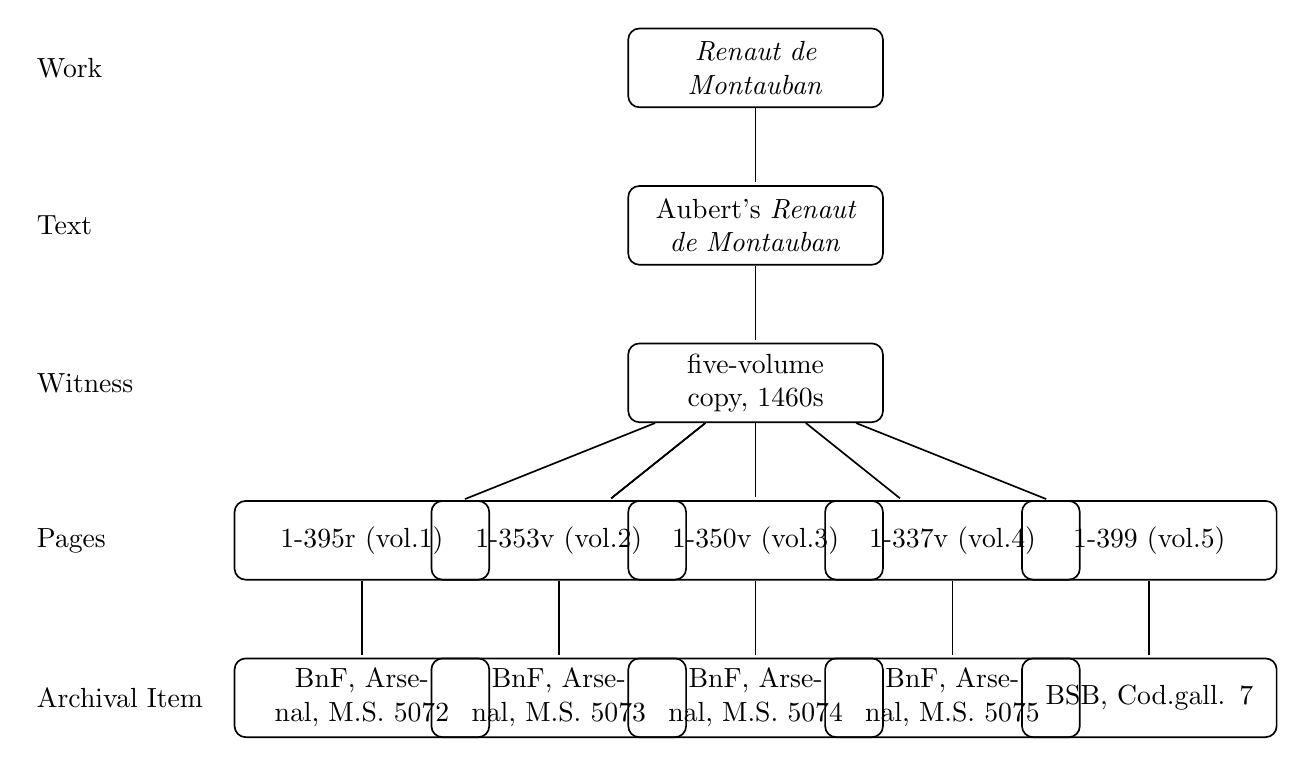
\begin{tikzpicture}[-,shorten >=1pt,auto,node distance=2cm,semithick]
\tikzstyle{every state}=[fill=red,draw=none,text=white]

\node[s] (Wk) {\textit{Renaut de Montauban}};
\node [left=6cm, text width=3cm] at (Wk) {Work};

\node[s] (T) [below of=Wk] {Aubert's \textit{Renaut de Montauban}};
\node [left=6cm, text width=3cm] at (T) {Text};

\node[s] (W) [below of=T] {five-volume copy, 1460s};
\node [left=6cm, text width=3cm] at (W) {Witness};

\node[s] (V3) [below of=W] {1-350v (vol.3)};
\node[s] (V2) [left of=V3, xshift=-0.5cm] {1-353v (vol.2)};
\node[s] (V1) [left of=V2, xshift=-0.5cm] {1-395r (vol.1)};
\node[s] (V4) [right of=V3, xshift=0.5cm] {1-337v (vol.4)};
\node[s] (V5) [right of=V4, xshift=0.5cm] {1-399 (vol.5)};
\node [left=1cm, text width=3cm] at (V1) {Pages};

\node[s] (D1) [below of=V1] {BnF, Arsenal, M.S. 5072};
\node[s] (D2) [below of=V2] {BnF, Arsenal, M.S. 5073};
\node[s] (D3) [below of=V3] {BnF, Arsenal, M.S. 5074};
\node[s] (D4) [below of=V4] {BnF, Arsenal, M.S. 5075};
\node[s] (D5) [below of=V5] {BSB, Cod.gall. 7};
\node [left=1cm, text width=3cm] at (D1) {Archival Item};

\path[every node/.style={font=\sffamily\small}]
    (Wk) edge node [right] {} (T)
    (T) edge node [right] {} (W)
    (W) edge node [right] {} (V1)
    (W) edge node [right] {} (V2)
    (W) edge node [right] {} (V2)
    (W) edge node [right] {} (V3)
    (W) edge node [right] {} (V4)
    (W) edge node [right] {} (V5)
    (V1) edge node [right] {} (D1)
    (V2) edge node [right] {} (D2)
    (V3) edge node [right] {} (D3)
    (V4) edge node [right] {} (D4)
    (V5) edge node [right] {} (D5)
    ;

\end{tikzpicture}
    \caption{Provisionary model of \textit{Renaut de Montauban} case.}
    \label{fig:RenautFinal}
    \end{center}
\end{figure}

It is necessary to introduce the intervening \textit{Pages} entity between the \textit{Witness} and the \textit{Item}. The reason is that an archival \textit{Item} may contain more than one \textit{Witness}. This happens to not be the case with \textit{Renaut de Montauban}. Each of the \textit{Items} contains nothing but its part of the \textit{Witness}. However, our second test case does involve manuscripts that transmit \textit{Witnesses} of more than one \textit{Work}, which will demonstrate the need for further development of the preexisting models.

\subsection{\textit{Chanson d'Aspremont} and the lost manuscript}

In April 1586, a notary named François Daunys certified who owned and leased what properties around the neighboring villages of Le Mazet, Fournels, and La Vachelerie, in what is today the Lozère \textit{département} of France.\footcite[][cxii]{camps2016} In the years that followed, notaries and others in the region kept track of the legal agreement, which eventually made its way into the Archives départementales de la Lozère. Around 1883, archivist Ferdinand André noticed the cover protecting the 1586 contract was an old bifolio, a piece of parchment folded in half, that had been cut from the quire of a manuscript. André then observed that each half of the biofolio contained part of a \textit{chanson de geste}, which he presumed dated from the thirteenth-century. André communicated his discovery to his colleagues and the fragments, being separated from the sixteenth-century legal document, were sent to the Bibliothèque nationale de France (BNF), where they are conserved today in a nineteenth-century collection of Medieval fragments.

The folded parchment that André discovered makes up the seventh and eighth folios of BNF, nouvelles aquisitions français (NAF) 5094. Each side's contents are not of the same \textit{chanson}, though they do come from the same original manuscript. Thus, in our adapted version of the FRBR data model, informed by Sahle's \textit{Textrad}, the composite BNF NAF 5094 manuscript would upwardly relate to two \textit{Pages} entities, one which begins on 7r and ends on 7v, and the other which begins on 8r and ends on 8v. Each \textit{Pages} entity would then relate to its own \textit{Witness}, because each folio is the fragment of a different \textit{Text} of a different \textit{Work}. Figure \ref{fig:BNFNAF5094} illustrates these relationships.

\begin{figure}[ht]
    \begin{center}
        \tikzstyle{s} = [rectangle, rounded corners, minimum width=2cm, text width=3cm, minimum height=1cm, text centered, draw=black]
\tikzstyle{arrow} = [thick,->,>=stealth]
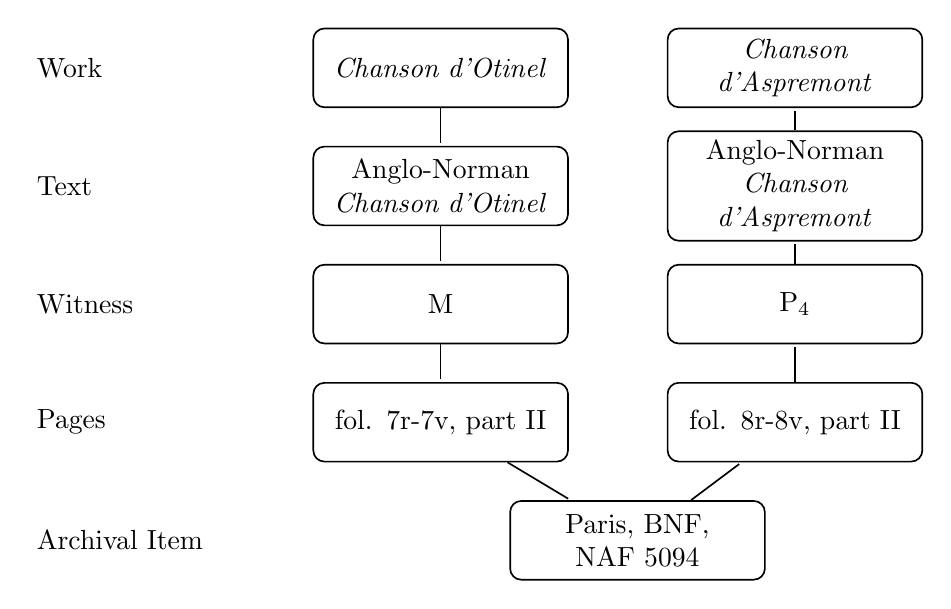
\begin{tikzpicture}[-,shorten >=1pt,auto,node distance=1.5cm,semithick]
\tikzstyle{every state}=[fill=red,draw=none,text=white]


\node[s] (WorkOtinel) {\textit{Chanson d'Otinel}};
\node[s] (WorkAspremont) [right of=WorkOtinel, xshift=3cm] {\textit{Chanson d'Aspremont}};
\node [left=2cm, text width=3cm] at (WorkOtinel) {Work};

\node[s] (ExpressionOtinel) [below of=WorkOtinel] {Anglo-Norman \textit{Chanson d'Otinel}};
\node[s] (ExpressionAspremont) [below of=WorkAspremont] {Anglo-Norman \textit{Chanson d'Aspremont}};
\node [left=2cm, text width=3cm] at (ExpressionOtinel) {Text};

\node[s] (ManifestationOtinel) [below of=ExpressionOtinel] {M};
\node[s] (ManifestationAspremontC) [below of=ExpressionAspremont] {P\textsubscript{4}};
% \node[s] (ManifestationAspremontP) [below of=ExpressionAspremont, xshift=2cm] {P\textsubscript{4}};
\node [left=2cm, text width=3cm] at (ManifestationOtinel) {Witness};

\node[s] (PagesOtinel) [below of=ManifestationOtinel] {fol. 7r-7v, part II};
\node[s] (PagesAspremontC) [below of=ManifestationAspremontC] {fol. 8r-8v, part II};
% \node[s] (PagesAspremontP) [below of=ManifestationAspremontP] {fol. 1r-2a};
\node [left=2cm, text width=3cm] at (PagesOtinel) {Pages};

\node[s] (ItemBNF) [below of=PagesOtinel, xshift=2.5cm] {Paris, BNF, NAF 5094};
% \node[s] (ItemCF) [below of=PagesAspremontP, xshift=-2cm] {Clermont-Ferrand, Arch. Dép., I F2};
\node[left=4.5cm, text width=3cm] at (ItemBNF) {Archival Item};

\path[every node/.style={font=\sffamily\small}]
    (WorkOtinel) edge node [right] {} (ExpressionOtinel)
    (ExpressionOtinel) edge node [right] {} (ManifestationOtinel)
    (ManifestationOtinel) edge node [right] {} (PagesOtinel)
    (PagesOtinel) edge node [right] {} (ItemBNF)
    (ItemBNF) edge node [right] {} (PagesAspremontC)
    (PagesAspremontC) edge node [right] {} (ManifestationAspremontC)
    (ManifestationAspremontC) edge node [right] {} (ExpressionAspremont)
    (ExpressionAspremont) edge node [right] {} (WorkAspremont)
    ;

% \path[every node/.style={font=\sffamily\small}]
%     (ExpressionAspremont) edge node [right] {} (ManifestationAspremontP)
%     (ManifestationAspremontP) edge node [right] {} (PagesAspremontP)
%     (PagesAspremontP) edge node [right] {} (ItemCF)
% ;

\end{tikzpicture}
    \end{center}
    \caption{Provisionary model of \textit{chansons de geste} in BNF NAF 5094.}
    \label{fig:BNFNAF5094}
\end{figure}

\subsubsection{The \textit{Attested Document}}

There is a glaring problem with the modeling in Figure \ref{fig:BNFNAF5094}. As it stands, The provisionary model suggestes that everything in BNF NAF 5094 was transmitted together, the \textit{Chanson d'Otinel}, the \textit{Chanson d'Aspremont}, and a fragment of the \textit{Roman de la Rose} which follows on folios 9 and 10.  We can prevent such an incorrect inference by noting the \textit{Archival Item} is a ``false'' manuscript \brackettext{\textit{factice}}, meaning it consists of writings that have been belatedly compiled together. However, preventing a false positive still does not solve the problem because we want to also know that the biofolio now on the seventh and eighth pages of BNF NAF 5094 was part of one manuscript. We need another entity, the \textit{Attested Document}.

While the \textit{Archival Item} links \textit{Witnesses} M and P\textsubscript{4} by virtue of their current conservation status, the \textit{Attested Document} unites them by virtue of scholarly argumentation that claims they were initially transmitted together. More detail about our test case of the \textit{Chanson d'Aspremont} reveals why an \textit{Attested Document} entity is so crucial. In the 1880s, while François André was sharing his discovery about the \textit{Chanson d'Otinel} and \textit{Chanson d'Aspremont} fragments in the Archives départementales de la Lozère, archivist Paul Meyer noted that the archives of a nearby French \textit{département}, the Puy-de-Dôme, also had a fragment of the \textit{Chanson d'Aspremont} that was being used to cover some records in their collection. Unlike the Lozère archives, the Puy-de-Dôme archives did not give the Bibliothèque nationale de France their fragment of the \textit{Chanson d'Aspremont}. Today, one can consult it at the Archives départementales de Clermont-Ferrand under the shelfmark I F2.

%JBC: pas sûr de tout comprendre dans la formulation dans les lignes qui précèdent ou suivent.
% It's not completely a coincidence that M and P4 are in the same volumes: they were written on the same bifolio, taken from the same original quire -- sort of like a folder, that's why it was so easy to use them to store archival contracts
%Moreover, the original volume (attested document) was not necessarily composite (composite volume means "Volume formé par la réunion d'unités codicologiques indépendantes", https://codicologia.irht.cnrs.fr/theme/liste_theme/143#tr-302; where 'unité codicologique' means "Volume, partie de volume ou ensemble de volumes dont l'exécution peut être considérée comme une opération unique, réalisée dans les mêmes conditions de lieu, de temps et de technique."). It was more likely that it was a 'Recueil homogène' = 'homogeneous collection', which means 'Ensemble de textes indépendants copiés en un même volume par une même personne, dans un même lieu ou à une même époque', https://codicologia.irht.cnrs.fr/theme/liste_theme/431#tr-878
%JBC: On the other hand, the Clermont-Ferrand fragment is not in the same volume today at all, but in the AD, at Clermont.

The updated provisional data model illustrated in Figure \ref{fig:AspremontCFBNF} allows us to recognize the attested coexistence of the three fragments in a now-lost manuscript. Because the missing document is not conserved as such anywhere, it lacks a clear identifier like the \textit{Archival Items} that have shelfmarks. To compensate, we generate a name that concatenates the \textit{Attested Document's} alleged parts. The known copies of the two \textit{chansons de geste}, \textit{Witnesses} M and P\textsubscript{4}, bypass their \textit{Pages} entities and meet one another directly in the \textit{Attested Document}.

\begin{figure}[ht]
    \begin{center}
        \tikzstyle{s} = [rectangle, rounded corners, minimum width=2cm, text width=3cm, minimum height=1cm, text centered, draw=black]
\tikzstyle{arrow} = [thick,->,>=stealth]
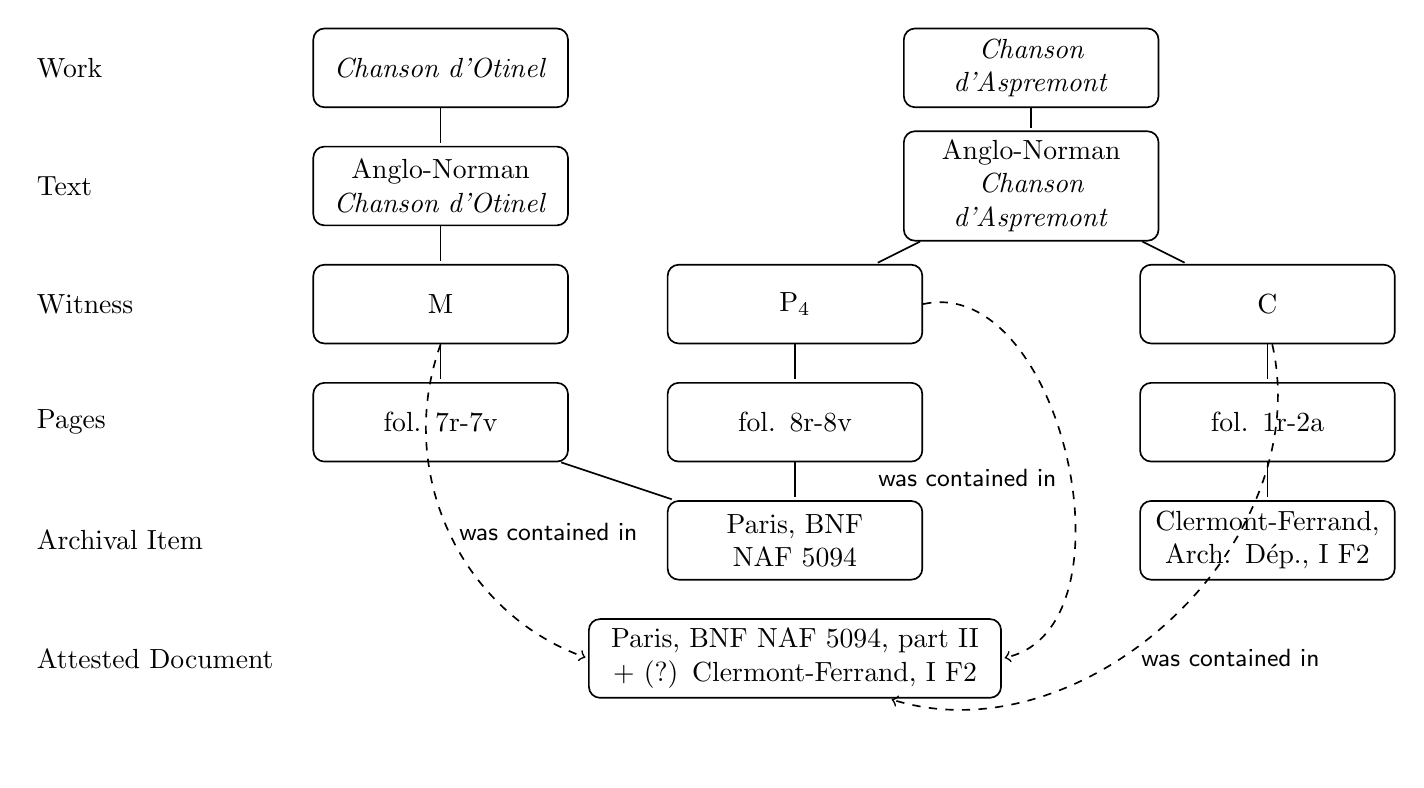
\begin{tikzpicture}[-,shorten >=1pt,auto,node distance=1.5cm,semithick]
\tikzstyle{every state}=[fill=red,draw=none,text=white]

\node[s] (Text) [] {Anglo-Norman \textit{Chanson d'Aspremont}};

\node[s] (P) [below of=Text, xshift=-3cm] {P\textsubscript{4}};
\node[s] (C) [below of=Text, xshift=3cm] {C};
\node[s] (M) [left of=P, xshift=-3cm] {M};
\node[s] (TextOtinel) [above of=M] {Anglo-Norman \textit{Chanson d'Otinel}};
\node [left=2cm, text width=3cm] at (TextOtinel) {Text};
\node [left=2cm, text width=3cm] at (M) {Witness};

\node[s] (WorkOtinel) [above of=TextOtinel] {\textit{Chanson d'Otinel}};
\node[s] (Work) [above of=Text] {\textit{Chanson d'Aspremont}};
\node [left=2cm, text width=3cm] at (WorkOtinel) {Work};

\node[s] (PagesP) [below of=P] {fol. 8r-8v};
\node[s] (PagesC) [below of=C] {fol. 1r-2a};
\node[s] (PagesM) [below of=M] {fol. 7r-7v};
\node [left=2cm, text width=3cm] at (PagesM) {Pages};

\node[s] (BNF) [below of=PagesP] {Paris, BNF NAF 5094};
\node[s] (CF) [below of=PagesC] {Clermont-Ferrand, Arch. Dép., I F2};
\node [left=6.5cm, text width=3cm] at (BNF) {Archival Item};

\node[s] (AttestedDoc) [below of=BNF, text width=5cm] 
{Paris, BNF NAF 5094, part II + (?) Clermont-Ferrand, I F2};
\node [left=5.5cm, text width=4cm] at (AttestedDoc) {Attested Document};

\path[every node/.style={font=\sffamily\small}]
  (Text) edge node [right] {} (P)
  (Work) edge node [right] {} (Text)
  (WorkOtinel) edge node [right] {} (TextOtinel)
  (Text) edge node [right] {} (C)
  (P) edge node [right] {} (PagesP)
  (C) edge node [right] {} (PagesC)
  (PagesP) edge node [right] {} (BNF)
  (PagesC) edge node [right] {} (CF)
  (P) edge[dashed, ->, bend left=90] node [left, yshift=-0.25cm] {was contained in} (AttestedDoc)
  (C) edge[dashed, ->, bend left=60] node [right, xshift=-0.5cm, yshift=-0.5cm] {was contained in} (AttestedDoc)
  (TextOtinel) edge node [right] {} (M)
  (M) edge node [right] {} (PagesM)
  (PagesM) edge node [right] {} (BNF)
  (M) edge[dashed, ->, bend right=45] node [right] {was contained in} (AttestedDoc)
  ;

\end{tikzpicture}
    \end{center}
    \caption{Provisionary model of \textit{chansons de geste} in BNF, NAF 5094 and Clermont-Ferrand I F2.}
    \label{fig:AspremontCFBNF}
\end{figure}

The model shown in Figure \ref{fig:AspremontCFBNF} perpetuates sigla (P\textsubscript{4}, C) that philologists have historically given to each fragment and communicates that both \textit{Witnesses} were likely transmitted together in the same manuscript (the \textit{Attested Document}). It does not, however, document the hypothesis that P\textsubscript{4} and C are in fact two parts of the same \textit{Witness}. While it is good to demonstrate that a manuscript contained copies of both the \textit{Chanson d'Otinel} and the \textit{Chanson d'Aspremont}, this is not sufficient. We do not want to lose the related theory that the verses of the Anglo-Norman \textit{Chanson d'Aspremont}, which are preserved today in two different fragments, are in fact different parts of one copy. Put another way, the model as is risks suggesting that the \textit{Attested Document} transmitted one copy of the Anglo-Norman \textit{Chanson d'Otinel} and two copies of the Anglo-Norman \textit{Chanson d'Aspremont}. The evidence does not suggest this latter claim.\footnote{Some scholars do argue that, originally, the manuscript for which \textit{Witness} P\textsubscript{4} was written was at some point damaged and it lost some of the leaves that presented the end of the \textit{Chanson d'Aspremont}, making the original \textit{Witness} into a fragment. Thus, the \textit{Witnesses} P\textsubscript{4} and C are not of the same original document because \textit{Witness} C was written after P\textsubscript{4} to replace some of the lost leaves. However, this theory, while interesting for the study of the \textit{Chanson d'Aspremont}, does not undermine the argument for why we need an \textit{Attested Document} entity because it still posits the existence of a lost manuscript that compiled the \textit{Witnesses} together.}
%JBC: the case here is even more complicated because some scholares have argued that C was posterior to M and P4: the original 'recueil homogène' would have lost some leaves that would have been redone at a later date and reintegrated in the 'recueil', to replace the damaged/missing ones.
%But I see you are discussing this later

\subsubsection{Inter-\textit{Witness} relationships}

% It is not enough to fuse the \textit{Witnesses} P\textsubscript{4} and C into one. On the one hand, we want the data model to preserve the status of existing \textit{Witnesses} as well as operate with the sigla philologists have historically given to archival fragments. In other words, we want to keep the \textit{Witness} entities seen in Figure \ref{fig:AspremontCFBNF}. On the other hand, the data model needs to be able to reveal that the two fragmentary \textit{Witnesses}, P\textsubscript{4} and C, are presumably parts of one fragmented \textit{Witness}.

The P\textsubscript{4} \textit{Witness} in BNF NAF 5094 does not start at the beginning of the \textit{Text}, meaning the Anglo-Norman version of the \textit{Chanson d'Asprmont}. As Jean-Baptiste Camps writes in his dissertation, the Paris fragment is likely missing about 85 verses of the beginning, after which it presents 395 verses of the \textit{Text}.\footcite[][xcvi]{camps2016} The Clermont-Ferrand (C) fragment presents the end of the \textit{Text}; it would total 384 verses if not for edges of its pages being cut. In putting the two fragments together, they miss about 85 verses at the beginning and 9606 in the middle. Their content does not overlap and, based on handwriting and language, there is reason to believe they were produced as one copy (\textit{Witness}) of the Anglo-Norman \textit{Chanson d'Aspremont}.

\begin{table}[ht]
    \begin{center}
    \begin{tabular}{c||cccc}
        \textit{Witness} & initial lacuna & P\textsubscript{4} text & middle lacuna & C text \\
        \hline
        \hline
        P\textsubscript{4} + C & & 395 & & 377 [384] \\
        Ch & 84 & 415 & 9606 & 388
    \end{tabular}
    \end{center}
\caption{Reproduction of the comparison between the number of verses in the complete \textit{Witness} Ch and the fragments P\textsubscript{4} and C, originally published in the dissertation of Jean-Baptiste Camps\footcite[Table 1.3.][xcvii]{camps2016}}
\label{tab:CampsAspremont}
\end{table}

Why not create another entity, the \textit{Attested Witness}, like the \textit{Attested Document}?\footnotemark\footnotetext{An example of such an entity is suggested in the first row of Table \ref{tab:CampsAspremont}, bearing the name ``P\textsubscript{4} + C.''} The latter is justified because the \textit{Attested Document} is ontologically different than the \textit{Archival Item}. The \textit{Archival Item} is a physical object in the world, which can be photographed and damaged. The \textit{Attested Document} is an historical claim asserting that a text object was once produced and existed in the world, but has not been conserved as such. An \textit{Attested Witness} and a regular \textit{Witness} are too ontologically similar; they are both philological claims that the sequence of characters inscribed on the pages of a document intentionally represents the linguistic content of a \textit{Text}, or of a text-as-linguistic-content as Sahle puts it. The difference between the attested \textit{Witness} ``P\textsubscript{4} + C'' and the \textit{Witnesses} P\textsubscript{4} and C is not categorical. Both are essentially historical claims. It does not justify the creation of a new entity.

A more efficient way to make legible in the data model the theoretical \textit{Witness} ``P\textsubscript{4} + C'' is to build that information into attributes of the \textit{Witnesses} that constitute it. The provisional model in Figure \ref{fig:WitnessRelations} shows how a \textit{Witness} that is a fragment can relate to another \textit{Witness} fragment via the attribute ``is preceded by fragment.'' In the \textit{Chanson d'Aspremont} case, the \textit{Witness} C would refer to P\textsubscript{4} in its field ``is preceded by fragment.'' \textit{Witness} P\textsubscript{4} would not have any value assigned to the attribute ``is preceded by fragment'' because it is the root of a sequence of \textit{Witness} fragments.\footnote{The fact that the P\textsubscript{4} \textit{Witness} would not have any value in its ``is preceded by fragment'' attribute, yet it has the status of ``fragment,'' could mean one of two things: (a) it is the only known fragment of that \textit{Witness}, or (b) that it is the root in a sequence of fragments that constitute one attested \textit{Witness}. To determine which is the case, one would need to identify roots of sequences by grouping all the \textit{Witnesses} based on other fragment \textit{Witnesses} referenced in the attribute ``is preceded by.''} 

However, we also know that \textit{Witness} M of the \textit{Chanson d'Otinel} was positioned before the \textit{Chanson d'Aspremont} in the \textit{Attested Document}. To show this, we link the root fragment \textit{Witness} P\textsubscript{4} to the \textit{Witness} that precedes it, M, with the attribute ``is preceded by witness.'' The relationships between \textit{Witnesses} as established by scribes consulting different manuscripts as models when composing a new version of a \textit{Text}, the subject of stemmatology, are not the focus of these inter-\textit{Witness} relationships. As discussed in Section \ref{sub:Graph}, the proposed relational framework is focused on curating and enriching data about the literary content and archival evidence of the corpus. How that evidence, the \textit{Witnesses}, were composed is best modeled in a graph framework.

\begin{figure}[ht]
    \begin{center}
        \tikzstyle{s} = [rectangle, rounded corners, minimum width=2cm, text width=3cm, minimum height=1cm, text centered, draw=black]
\tikzstyle{arrow} = [thick,->,>=stealth]
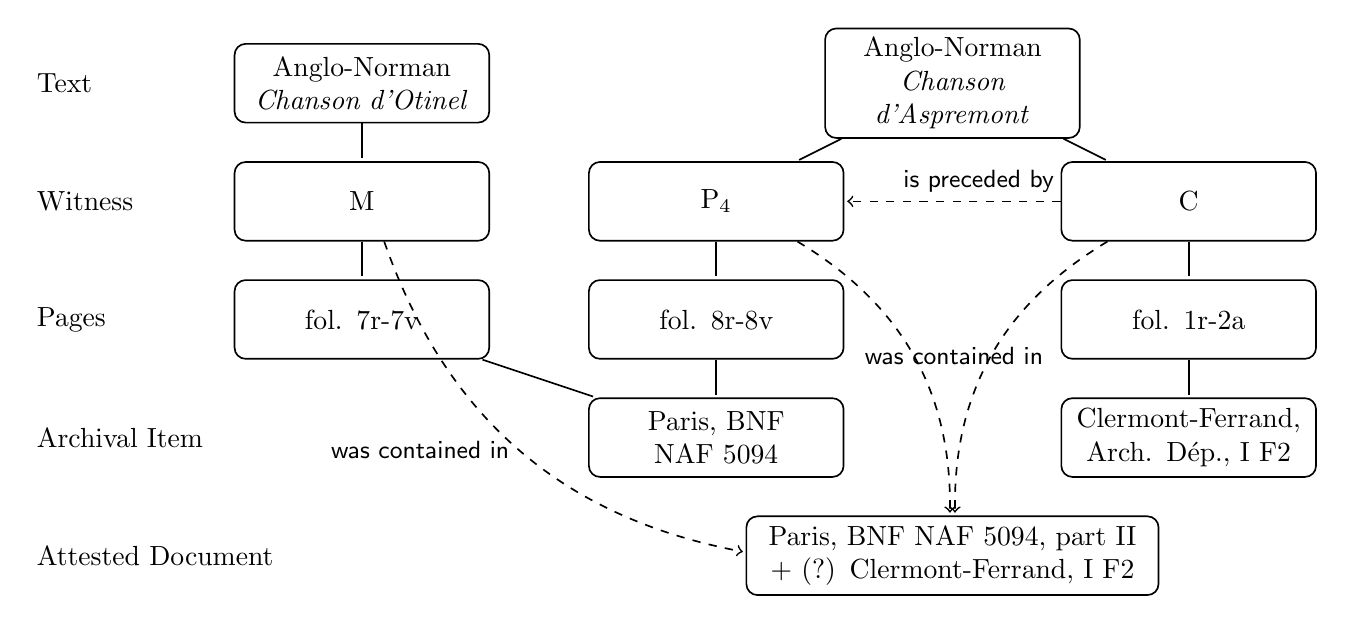
\begin{tikzpicture}[-,shorten >=1pt,auto,node distance=1.5cm,semithick]
\tikzstyle{every state}=[fill=red,draw=none,text=white]

\node[s] (Text) [] {Anglo-Norman \textit{Chanson d'Aspremont}};

\node[s] (P) [below of=Text, xshift=-3cm] {P\textsubscript{4}};
\node[s] (C) [below of=Text, xshift=3cm] {C};
\node[s] (M) [left of=P, xshift=-3cm] {M};
\node[s] (TextOtinel) [above of=M] {Anglo-Norman \textit{Chanson d'Otinel}};
\node [left=1cm, text width=3cm] at (TextOtinel) {Text};
\node [left=1cm, text width=3cm] at (M) {Witness};

\node[s] (PagesP) [below of=P] {fol. 8r-8v};
\node[s] (PagesC) [below of=C] {fol. 1r-2a};
\node[s] (PagesM) [below of=M] {fol. 7r-7v};
\node [left=1cm, text width=3cm] at (PagesM) {Pages};

\node[s] (BNF) [below of=PagesP] {Paris, BNF NAF 5094};
\node[s] (CF) [below of=PagesC] {Clermont-Ferrand, Arch. Dép., I F2};
\node [left=5.5cm, text width=3cm] at (BNF) {Archival Item};

\node[s] (AttestedDoc) [below of=BNF, xshift=3cm, text width=5cm] 
{Paris, BNF NAF 5094, part II + (?) Clermont-Ferrand, I F2};
\node [left=7.5cm, text width=4cm] at (AttestedDoc) {Attested Document};

\path[every node/.style={font=\sffamily\small}]
  (Text) edge node [right] {} (P)
  (Text) edge node [right] {} (C)
  (P) edge node [right] {} (PagesP)
  (C) edge node [right] {} (PagesC)
  (PagesP) edge node [right] {} (BNF)
  (PagesC) edge node [right] {} (CF)
  (P) edge[dashed, ->, bend left=30] node [right, xshift=-0.75cm] {was contained in} (AttestedDoc)
  (C) edge[dashed, ->, bend right=30] node [right] {} (AttestedDoc)
  (C) edge[dashed, ->] node [right, xshift=-0.75cm, yshift=0.25cm] {is preceded by} (P)
  (TextOtinel) edge node [right] {} (M)
  (M) edge node [right] {} (PagesM)
  (PagesM) edge node [right] {} (BNF)
  (M) edge[dashed, ->, bend right=30] node [left] {was contained in} (AttestedDoc)
  ;

\end{tikzpicture}
    \end{center}
    \caption{Relationships between \textit{Witnesses} and neighboring entities in provisional model.}
    \label{fig:WitnessRelations}
\end{figure}

%JBC: to be discussed. I can see two points:
% 1. order of witnesses in the original 'attested document' (in this case, Otinel, then Aspremont, and P4 before C)
% 2. witnesses that may or may not be the same, and in that case, in which order (could also be deduced by the order of verses, if we were to store that information)

